\documentclass[a4paper,12pt,leqno]{article}
\usepackage[utf8]{inputenc}
\usepackage[T1]{fontenc}
\usepackage[polish]{babel}
\usepackage{amsmath}
\usepackage{a4wide}
\usepackage{graphicx}
\usepackage{subfig}
\usepackage{wrapfig}
\usepackage{program}

\title{\textbf{Algorytmy ewolucyjne}\\
       {\Large Raport z zadania pierwszego}\\[-1ex]}
\author{Karol Konaszyński i Wiktor Janas}
\date{Wrocław, dnia \today\ r.}

\begin{document}
\maketitle

\newcommand{\grad}{\mathrm{grad}}
\newcommand{\avg}{\mathrm{avg}}
\newcommand{\dist}{\mathrm{dist}}
\newcommand{\median}{\mathrm{median}}
\newcommand{\target}{\mathrm{target}}
\newcommand{\RETURN}{|return|\ }

\section{Abstrakt}

Hasłem przewodnim naszej pracy jest: Zastosowanie algorytmów ewolucyjnych do rozpoznawania obrazów. 
Problem rozpoznawania obrazów jest niezmiernie powszechnie spotykany; od analizy zdjęć satelitarnych poprzez monitorowania ruchu drogowego, po przemysł filmowy. 
Z drugiej strony jednak stanowi poważne wyzwanie dla informatyki, gdyż okazuje się niezwykle trudnym z powodu sposobu, 
w jaki ludzki mózg przetwarza i rozpoznaje obrazy. Przede wszystkim, wyzwaniem jest jednak precyzyjne jego sformułowanie; 
chodzi mianowicie o pojmowanie słowa ,,rozpoznawanie''. Nasza interpretacja niniejszego zagadnienia polega na rozstrzygnięciu, 
do jakiego obiektu ,,podobny'' jest kształtem przedmiot znajdujący się na obrazie. 
Przy tym rozpatrujemy tylko obrazy czarnobiałe. Tutaj ograniczymy się do takiego sformułowania, zostawiając słowo ,,podobny'' jako określenie intuicyjne. 

\section{Opis podejścia do problemu}
Przyjęliśmy następujący schemat. Mamy daną bazę obrazów (obrazy ,,bazowe'') o zadanych nazwach (to znaczy, że wiemy, co przedstawiają) 
i dla każdego obrazka, który chcemy rozpoznać (,,zapytania''), przyrównujemy do niego wszystkie obrazków bazowych i znajdujemy ich odległość. 
Następnie spośród otrzymanych odległości, wybieramy najmniejszą i odpowiedzią dla tego zapytania jest nazwa obrazka minimalizującego tę odległość.
W tym akapicie skupimy się na szczegółach powyższego opisu.

\subsection{Znajdowanie punktów charakterystycznych}
Pierwszym etapem przetwarzania obrazka jest znalezienie na nim punktów charakterystycznych. Dla każdego punktu liczymy jego ,,miarę ciekawości''.
Mianowicie, dla danej skali d i kierunku $\alpha$ wyznaczamy gradient tego punktu w tę stronę; 
intuicyjnie, jest to różnica średnich jasności otoczenia tego piksela i jego otoczenia przesuniętego o d w stronę $\alpha$. 
Formalniej, niech $avg(x,y,d)$ oznacza średnią jasność obrazu w kwadracie o środku w (x,y) i boku długości d. Wówczas:
\[
\grad(x,y,d,\alpha) = \avg(x,y,d) - \avg(x+\sin(\alpha)d, y+\cos(\alpha)d, d)
\]
Dla danego kierunku, wyznaczamy średnią geometryczną gradientów dla określonego wektora skal. W naszej implementacji użyliśmy skal $d = 1, 3, 8$, 
zatem 
\[
\grad(x,y,\alpha ) = \sqrt[3]{\grad(x,y,1,\alpha ) \cdot \grad(x,y,3,\alpha ) \cdot \grad(x,y,8,\alpha )}
\]
[rysunek: dwa kwadraty na polu pikseli]
W ten sposób dostajemy, dla danego piksela, funkcję gradientu od kąta i badamy jej amplitudę. Jej wysokość to nasza szukana ,,miara ciekawości''.
Interesującą obserwacją jest to, że dla skali równej 1 funkcja którą otrzymujemy jest sklejeniem kilku funkcji polisinusoidalnych.
Heurystyka stojąca za tym algorytmem jest prosta - szukamy punktów, w których obszar (w miarę) jednokolorowy przechodzi w obszar o innym kolorze. 
Amplituda funkcji gradientu mówi właśnie to, jak w otoczeniu piksela zmienia się kolor. 
Należy jednak uwzględnić to, że niektóre zmiany sś jedynie lokalne. Aby więc wyeleminować ,,szum'', 
liczymy tę funkcję dla dwóch skal i mnożymy - jeżeli istotnie, zachodzi globalna zmiana koloru, nastąpi rezonans, 
gdy natomiast zmiana jest lokalna - funkcja większej skali ją ,,wyciszy''. Według naszej całkowicie subiektywnej oceny skale 1,3,8 spradzają się najlepiej.
To jednak nie jest koniec. Chcemy bowiem mieć coś więcej - określoną liczbę punktów charakterystycznych, 
które będą opisywały nam kształt obiektu. Liczba ta jest parametrem alogorytmu, najczęściej przyjmowaliśmy 50. Musimy zatem wybrać ten zbiór spośród wszystkich pikseli obrazka. 
Do tego celu zastosowaliśmy następujący algorytm: w każdym kolejnym kroku wybieramy najciekawszy piksel na obrazku i dodajemy go do zbioru punktów interesujących.
Nastepnie jego otoczenie oznaczamy jako tabu i powtarzamy procedurę tak długo, aż wszystkie punkty zostaną tabu. 
Aby określić wielkość tabu, zastosowaliśmy heurystykę: ,,im ciekawiej tym gęściej''. Mianowicie, 
wielkość tabu jest odwrotnie proporcjonalna do miary ciekawości punktu z pewnym współczynnikiem, który jest dobierany (na przykład za pomocą wyszukiwania binarnego)
tak, aby ostateczny zbiór punktów miał określoną wielkość.

\begin{figure}\centering
\subfloat[gradient, $d = 1$]{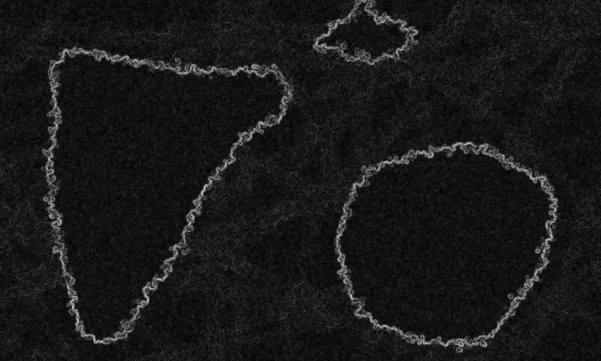
\includegraphics[width=6cm,keepaspectratio=true]{./noisy-grad-1.png}}\hspace{5mm}
\subfloat[gradient, $d = 3$]{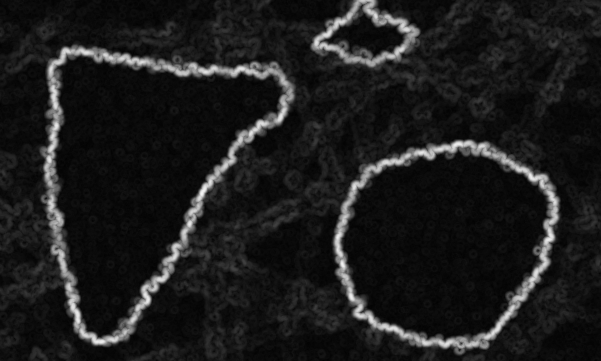
\includegraphics[width=6cm,keepaspectratio=true]{./noisy-grad-3.png}}\\
\subfloat[gradient, $d = 8$]{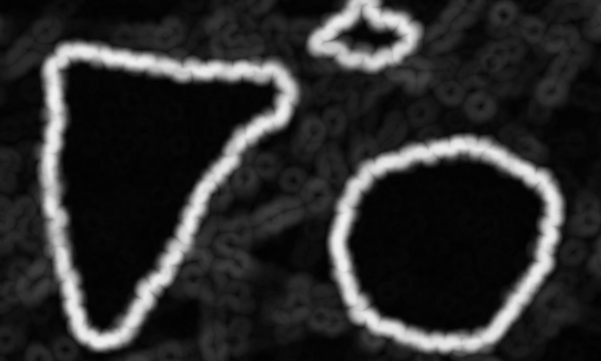
\includegraphics[width=6cm,keepaspectratio=true]{./noisy-grad-8.png}}\hspace{5mm}
\subfloat[gradient, łącznie]{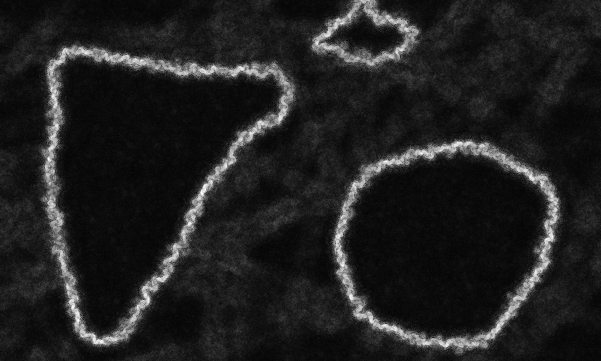
\includegraphics[width=6cm,keepaspectratio=true]{./noisy-grad.png}}\\
\subfloat[znalezione punkty]{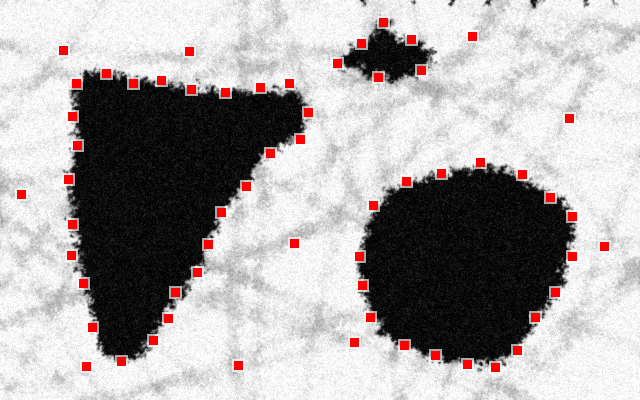
\includegraphics[width=6cm,keepaspectratio=true]{./noisy-pois.png}}
\caption{Proces wyszukiwania punktów charakterystycznych}
\end{figure}

\subsection{Zastosowanie ewolucji i kodowanie osobników}
Mając już punkty charakterystyczne, możemy zająć się badaniem podobienstwa obrazków. Mówimy, że obrazki są równoważne, jeżeli istnieje przekształcenie afiniczne 
przenoszące jeden na drugi. Miarą podobieństwa dwóch zbiorów punktów infimum, po wszystkich przekształceniach,
sumy ,,odległości,, jednego z nich od przekształconego drugiego oraz w drugą stronę. 
Odległość natomiast dwóch zbiorów definiujemy jako średnią odległość pomiędzy punktem z pierwszego zbioru a najbliższym mu punktem z drugiego, Formalniej,
\[
\mathrm{similar}(\bar{A}, \bar{B}) = \inf\{\textrm{dist}(\bar{A} - M\bar{B}) \text{afiniczne}\}
\]gdzie:
\[
\dist(\{a_1, \dots, a_m\}, \{b_1, \dots, b_n\}) = \frac{\sum_{i=1}^m \min_{j=1..n}(\|a_i - b_j\|)}{m} + \frac{\sum_{i=1}^n min_{j=1 \dots m}(\|b_i - a_j\|)}{n}
\]
Jednak aby znaleźć wielkość $\mathrm{similar}$ musimy znaleźć przekształcenie minimalizujące odległość. I tutaj zastosujemy ewolucję. 
Naszymi osobnikami będą macierze afiniczne, czyli macierze postaci:
$\begin{pmatrix}
\star & \star & \star \\
\star & \star & \star \\
0 & 0 & 1
\end{pmatrix}$, gdzie drugi minor główny jest złożeniem obrotu i skalowania, natomiast ostatnia kolumna odpowiada za translację.
Funkcją celu jest zatem 
\[
\target = -\dist(\bar{q}, M\bar{b})
\]
gdzie $\bar{q}$ jest wektorem punktów charakterystycznych obrazka z zapytania, zaś $\bar{b}$ - wektorem tychże dla obrazka z bazy.
Celem ewolucji jest zmaksymalizowanie funkcji celu, czyli znalezienie przekształcenia minimalizującego odległość.

\subsection{Ewolucja}
Do niniejszego problemu wykorzystaliśmy ideę Differential Evolution. Pseudokod funkcji wykonującej ewolucję wygląda następująco:
\begin{figure}
\begin{program}
\FUNCT |evolve| \BODY
    P := \{\}
    \FOR i := 1 \TO N \DO
        P := P + |random_translation|() * |random_rotation|() * |random_scaling|()
    \END
    \WHILE \NOT |termination_condition|() \DO
        \FOR i := 1 \TO N \DO
            |evaluate|(P_i)
        \END
        |sort|(P) 
        ~
        P := \set{P_i | i \leq N*|replace\_rate| }
        \FOR i := 1 \TO N*|replace_rate| \DO
            \IF |random|(|de_prop|)
                \THEN P := P + |de_crossover|(P);
                \ELSE P := P + |roulette_selection|(P); \FI
        \END
        ~
        \FOR i := 1 \TO N \DO 
            \IF |random|(|t_prop|)
	        \THEN P_i := |random_translation| * P_i; \FI
            \IF |random|(|s_prop|)
                \THEN P_i := |random_scaling| * P_i; \FI
            \IF |random|(|r_prop|)
                \THEN P_i := |random_rotation| * P_i; \FI
        \END
    \END
\END

\FUNCT |de_crossover| \BODY
    x1 := |roulette_selection|(P)
    x2 := |roulette_selection|(P),\; x1 \neq x2
    x3 := |roulette_selection|(P),\; x3 \neq x1,\; x3 \geq x2
    \RETURN x1 + (x3-x2) * f_\text{de}
\END

\FUNCT |termination_condition| \BODY
    \RETURN |generation_index| > G \vee
            |max_target|(|generation_index|, |generation_index|-K) \geq
            |max_target|(|generation_index|-K, |generation_index|-2*K)
\END
\end{program}
\end{figure}

Skomentuję krótko działanie powyższych funkcji. Najpierw odbywa się losowa inicjacja populacji z parametrem N. Następnie wchodzimy w pętlę ewolucji,
która wykonuje się aż nie zostanie spełniony warunek zakończenia.
W pętli, pierwszą rzeczą jest ewaluacja każdego osobnika, czyli znalezienie dla niego wartości $\target$. 
Potem następuje zastąpienie części populacji przez osobniki bądź otrzymane w wyniku krzyżowania DE (z określonym jako parametr prawdopodobieństwem),
bądź wybrane na zasadzie ruletki z całości populacji (zjawisko generational gap).
Na końcu działania ciała pętli następuje mutacja każdego osobnika, czyli przemnożenie go (z lewej strony) przez macierz losowego przesunięcia, 
skalowania bądź obrotu, z prawdopodobieństwami określonymi jako globalne parametry algorytmu.
Warunkiem zakończenia jest natomiast przekroczenie pewnej ilości pokoleń (parametr algorytmu, zwykle rzędu 200) bądź stwierdzeniem, 
że w czasie ostatnich K pokoleń nie nastąpiła poprawa w stosunku do poprzednich K pokoleń (K jest również parametrem). Precyzyjniej, najlepszy osobnik z ostatnich 
K pokoleń okazał się nielepszy niż najlepszy z poprzednich K pokoleń.

Skomentuję jeszcze dwa miejsca w tym algorytmie.
Krzyżowanie DE polega na wybraniu, na zasadzie ruletki, trzech różnych osobników $x_1, x_2, x_3$ a następnie utworzeniu z nich osobnika postaci
$x1 + f_\text{de}\cdot(x3-x2)$, gdzie $f_\text{de}$ jest także parametrem, zaś operacja dodawania i mnożenia jest zwykłą operacją dodawania macierzy 
i mnożenia ich przez skalar.
Ważną obserwacją którą poczyniliśmy jest to, że nie warto dokonywać losowych obrotów wokół (domyślnie) punktu (0,0), 
gdyż to spowoduje duże zmiany w położeniu punktów oddalonych od środka układu współrzędnych. Aby tego uniknąć, obroty i skalowania wykonujemy względem punktu wybranego z małego otoczenia
mediany zbioru punktów; konkretniej, względem punktu $(\median(\bar{X}), \median(\bar{Y}))$, gdzie $\bar{X}, \bar{Y}$ są zbiorami współrzędnych x, y punktów ze zbioru.

\begin{figure}\centering
\footnotesize\include{applemod-vs-fruits}\vspace{-2em}
\normalsize\caption{Dopasowanie owoców (\texttt{fruits}) do obróconego jabłka (\texttt{applemod}); uśrednione wyniki z dziesięciu uruchomień programu.}
\end{figure} 

\begin{figure}\centering
\footnotesize\include{square-vs-romb-popsize}\vspace{-2em}
\normalsize\caption{Wpływ rozmiaru populacji na ewolucję (dopasowanie \texttt{square} do \texttt{romb}); uśrednione wyniki z dziesięciu uruchomień programu.}
\end{figure}
\begin{figure}\centering
\footnotesize\include{square-vs-romb-deprop}\vspace{-2em}
\normalsize\caption{Wpływ prawdopodobieństwa krzyżowania na ewolucję (dopasowanie \texttt{square} do \texttt{romb}); uśrednione wyniki dziesięciu uruchomień programu.}
\end{figure}
\begin{figure}\centering
\footnotesize\include{square-vs-romb-surv}\vspace{-2em}
\normalsize\caption{Wpływ współczynnika przetrwania na ewolucję (dopasowanie \texttt{square} do \texttt{romb}); uśrednione wyniki dziesięciu uruchomień programu.}
\end{figure}

\begin{figure}\centering
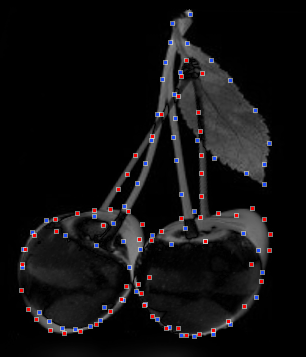
\includegraphics[width=6cm,keepaspectratio=true]{./cherries-match.png}
\caption{Dopasowanie \texttt{cherries} do \texttt{cherries6}}
\end{figure}


\begin{figure}\centering
\subfloat[Jabłko]{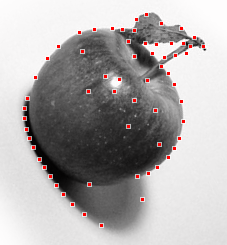
\includegraphics[width=6cm,keepaspectratio=true]{./apple-mod-pois.png}}
\subfloat[Wisienki]{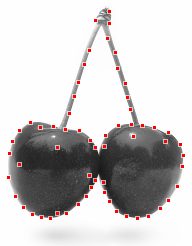
\includegraphics[width=6cm,keepaspectratio=true]{./cherries-pois.png}}\\
\subfloat[Trójliterówka]{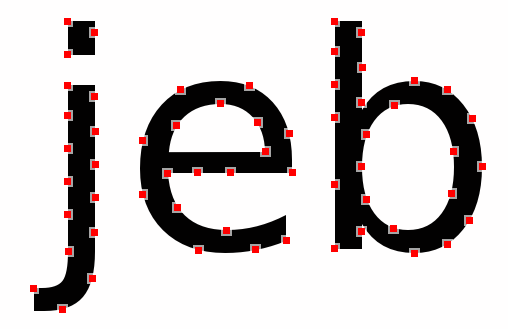
\includegraphics[width=6cm,keepaspectratio=true]{./jeb-pois.png}}
\caption{Obrazy testowe}
\end{figure}

\end{document}
